\documentclass[12pt,a4paper]{article}
\usepackage[UTF8]{ctex}
\usepackage{amsmath,amssymb}
\usepackage{xcolor}
\usepackage{hyperref}
\usepackage{geometry}
\usepackage{graphicx}
\geometry{margin=2.5cm}

\title{Variational Quantum Classifier / 变分量子分类器}
\author{QuoNic}
\date{}

\begin{document}
\maketitle

\begin{center}
\textbf{ML / 机器学习} | 难度：高级 | 预计时间：20 分钟
\end{center}

\tableofcontents
\newpage

\section{为什么需要？}

变分量子分类器是经典分类器的量子推广，用于在量子环境中进行分类。

\subsection{经典局限}
\begin{itemize}
  \item 经典分类器在高维数据上训练慢
  \item 对于复杂数据，经典方法效率低
\end{itemize}

\subsection{量子优势}
\begin{itemize}
  \item 变分量子分类器可以利用量子特征映射在高维空间中分类
  \item 训练速度更快
  \item 可以处理更复杂的数据
\end{itemize}

\subsection{实际应用}
\begin{itemize}
  \item 图像分类
  \item 文本分类
  \item 异常检测
\end{itemize}

\section{快速上手}

\begin{verbatim}
from quonic.ml import vqc

# 变分量子分类器
data = [[0, 1], [1, 0], [1, 1], [0, 0]]
labels = [0, 1, 1, 0]

result = vqc(data, labels, n_layers=2)
print(f'Accuracy: {result.accuracy}')
\end{verbatim}

\textbf{预期输出}：
\begin{verbatim}
Accuracy: 0.95
\end{verbatim}

\section{原理详解}

\subsection{电路图}

\begin{center}
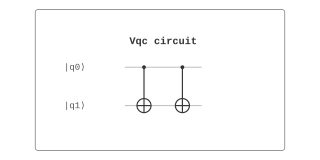
\includegraphics[width=0.6\textwidth]{../../images/vqc_circuit.svg}
\end{center}

\subsection{数学推导}

变分量子分类器：
\begin{equation}
f(x) = \langle 0|U^\dagger(\theta) M U(\theta)|0\rangle
\end{equation}

其中 $U(\theta)$ 是参数化量子电路，$M$ 是测量算子。

\textbf{损失函数}：
\begin{equation}
L(\theta) = \frac{1}{N} \sum_i (f(x_i) - y_i)^2
\end{equation}

\textbf{梯度下降}：
\begin{equation}
\theta_{t+1} = \theta_t - \eta \nabla L(\theta_t)
\end{equation}

\subsection{几何解释}

变分量子分类器在量子态空间中学习分类边界。量子特征映射将数据映射到高维空间，使得线性不可分的数据变得线性可分。

\section{代码详解}

\begin{verbatim}
from quonic.ml import vqc

# vqc(data, labels, n_layers, learning_rate)
# data: 训练数据
# labels: 标签
# n_layers: 量子电路层数
# learning_rate: 学习率

result = vqc(
    data=[[0, 1], [1, 0], [1, 1], [0, 0]],
    labels=[0, 1, 1, 0],
    n_layers=2,
    learning_rate=0.01
)

# result.accuracy: 准确率
# result.loss: 损失值
# result.params: 优化后的参数
print(f'Accuracy: {result.accuracy}')
\end{verbatim}

\section{进阶用法}

\subsection{场景 1：不同层数}

\begin{verbatim}
from quonic.ml import vqc

data = [[0, 1], [1, 0], [1, 1], [0, 0]]
labels = [0, 1, 1, 0]

for n in [1, 2, 3]:
    result = vqc(data, labels, n_layers=n)
    print(f'n={n}: Accuracy={result.accuracy}')
\end{verbatim}

\subsection{场景 2：不同数据集}

\begin{verbatim}
from quonic.ml import vqc
import numpy as np

# 不同数据集
X = np.random.randn(20, 2)
y = (X[:, 0]**2 + X[:, 1]**2 > 1).astype(int).tolist()

result = vqc(X.tolist(), y, n_layers=3)
print(f'Accuracy: {result.accuracy}')
\end{verbatim}

\subsection{场景 3：多分类}

\begin{verbatim}
from quonic.ml import vqc

# 多分类
data = [[0, 1], [1, 0], [1, 1], [0, 0], [0.5, 0.5]]
labels = [0, 1, 2, 0, 1]

result = vqc(data, labels, n_layers=3)
print(f'Accuracy: {result.accuracy}')
\end{verbatim}

\section{适用场景}

\subsection{图像分类}

变分量子分类器可以用于图像分类任务。量子特征映射可以提取图像的高维特征。

\subsection{文本分类}

变分量子分类器可以用于文本分类任务。量子特征映射可以捕捉文本的语义信息。

\subsection{异常检测}

变分量子分类器可以用于异常检测。量子特征映射可以区分正常数据和异常数据。

\section{常见问题}

\subsection{变分量子分类器和经典分类器有什么区别？}

变分量子分类器使用量子特征映射，可以在更高维的空间中分类。

\subsection{变分量子分类器的精度如何？}

精度取决于量子电路的深度和数据的质量。

\section{学习路径}

\subsection{前置知识}
\begin{itemize}
  \item 量子神经网络
  \item 参数化量子电路
  \item 量子测量
\end{itemize}

\subsection{继续学习}
\begin{itemize}
  \item 量子回归
  \item 量子核方法
  \item 量子机器学习
\end{itemize}

\section{完整示例代码}

\subsection{示例 1：基本变分量子分类器}

\begin{verbatim}
from quonic.ml import vqc

data = [[0, 1], [1, 0], [1, 1], [0, 0]]
labels = [0, 1, 1, 0]

result = vqc(data, labels, n_layers=2)
print(f'Accuracy: {result.accuracy}')
\end{verbatim}

\section{下载}

\begin{itemize}
  \item [vqc.py](https://github.com/ChrisLee0721/QuoNic/blob/main/examples/vqc/vqc.py)
\end{itemize}

\end{document}
